\section{Auswertung}
\label{sec:Auswertung}

\subsection{Amplitudenmodulierte Schwingung mit Ringmodulator}

Mit Hilfe der Schaltung aus Abbildung \ref{fig:???} wird eine Amplitudenmodulierte Schwingung erzeugt.
Diese so entstandene Schwebung ist in Abbildung \ref{fig:amplModOszi} zu sehen.

\begin{figure}[H]
  \centering
  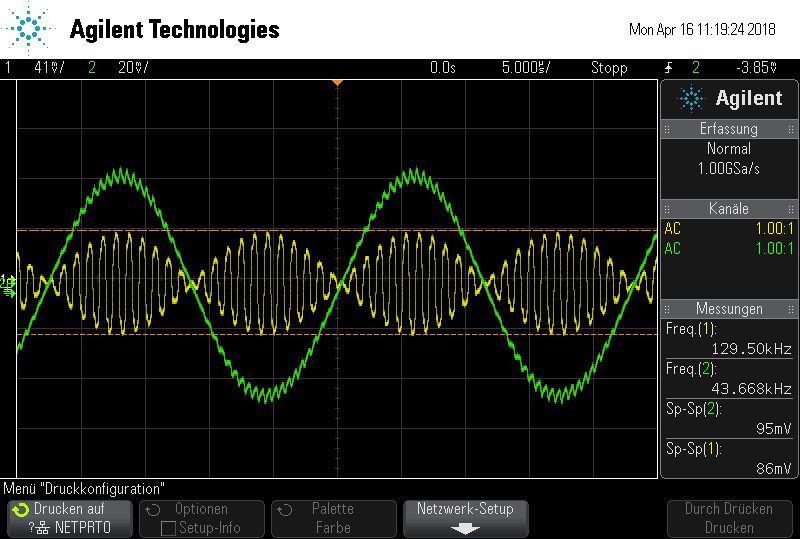
\includegraphics[width=\textwidth]{Oszi_Pics/amplModRing.png}
  \caption{Amplitudenmodulierte Schwingung(gelb) und Modulationsschwingung(grün) erzeugt mit Ringmodulator.}
  \label{fig:amplModOszi}
\end{figure}

Die mit dem Oszilloskop außerdem ausgemessenen Werte für die Frequenzen $\omega$ und Amplituden $U_\text{peak to peak}$ der Modulationsspannung $M$ und der Trägerspannung $T$ sind:

\begin{align*}
  \omega_\text{M} &= \SI{43.8(5)}{\kilo\hertz} & U_\text{M, ptp} &= \SI{95(1)}{\milli\volt}\\
  \omega_\text{T} &= \SI{970(1)}{\kilo\hertz} & U_\text{T, ptp} &= \SI{540(1)}{\milli\volt}.
\end{align*}

Die mit dem Frequenzspektrometer aufgenommenen Werte sind in den Bildern \ref{fig:b1}, \ref{fig:b2} und \ref{fig:b3} zu sehen.

\begin{figure}[H]
  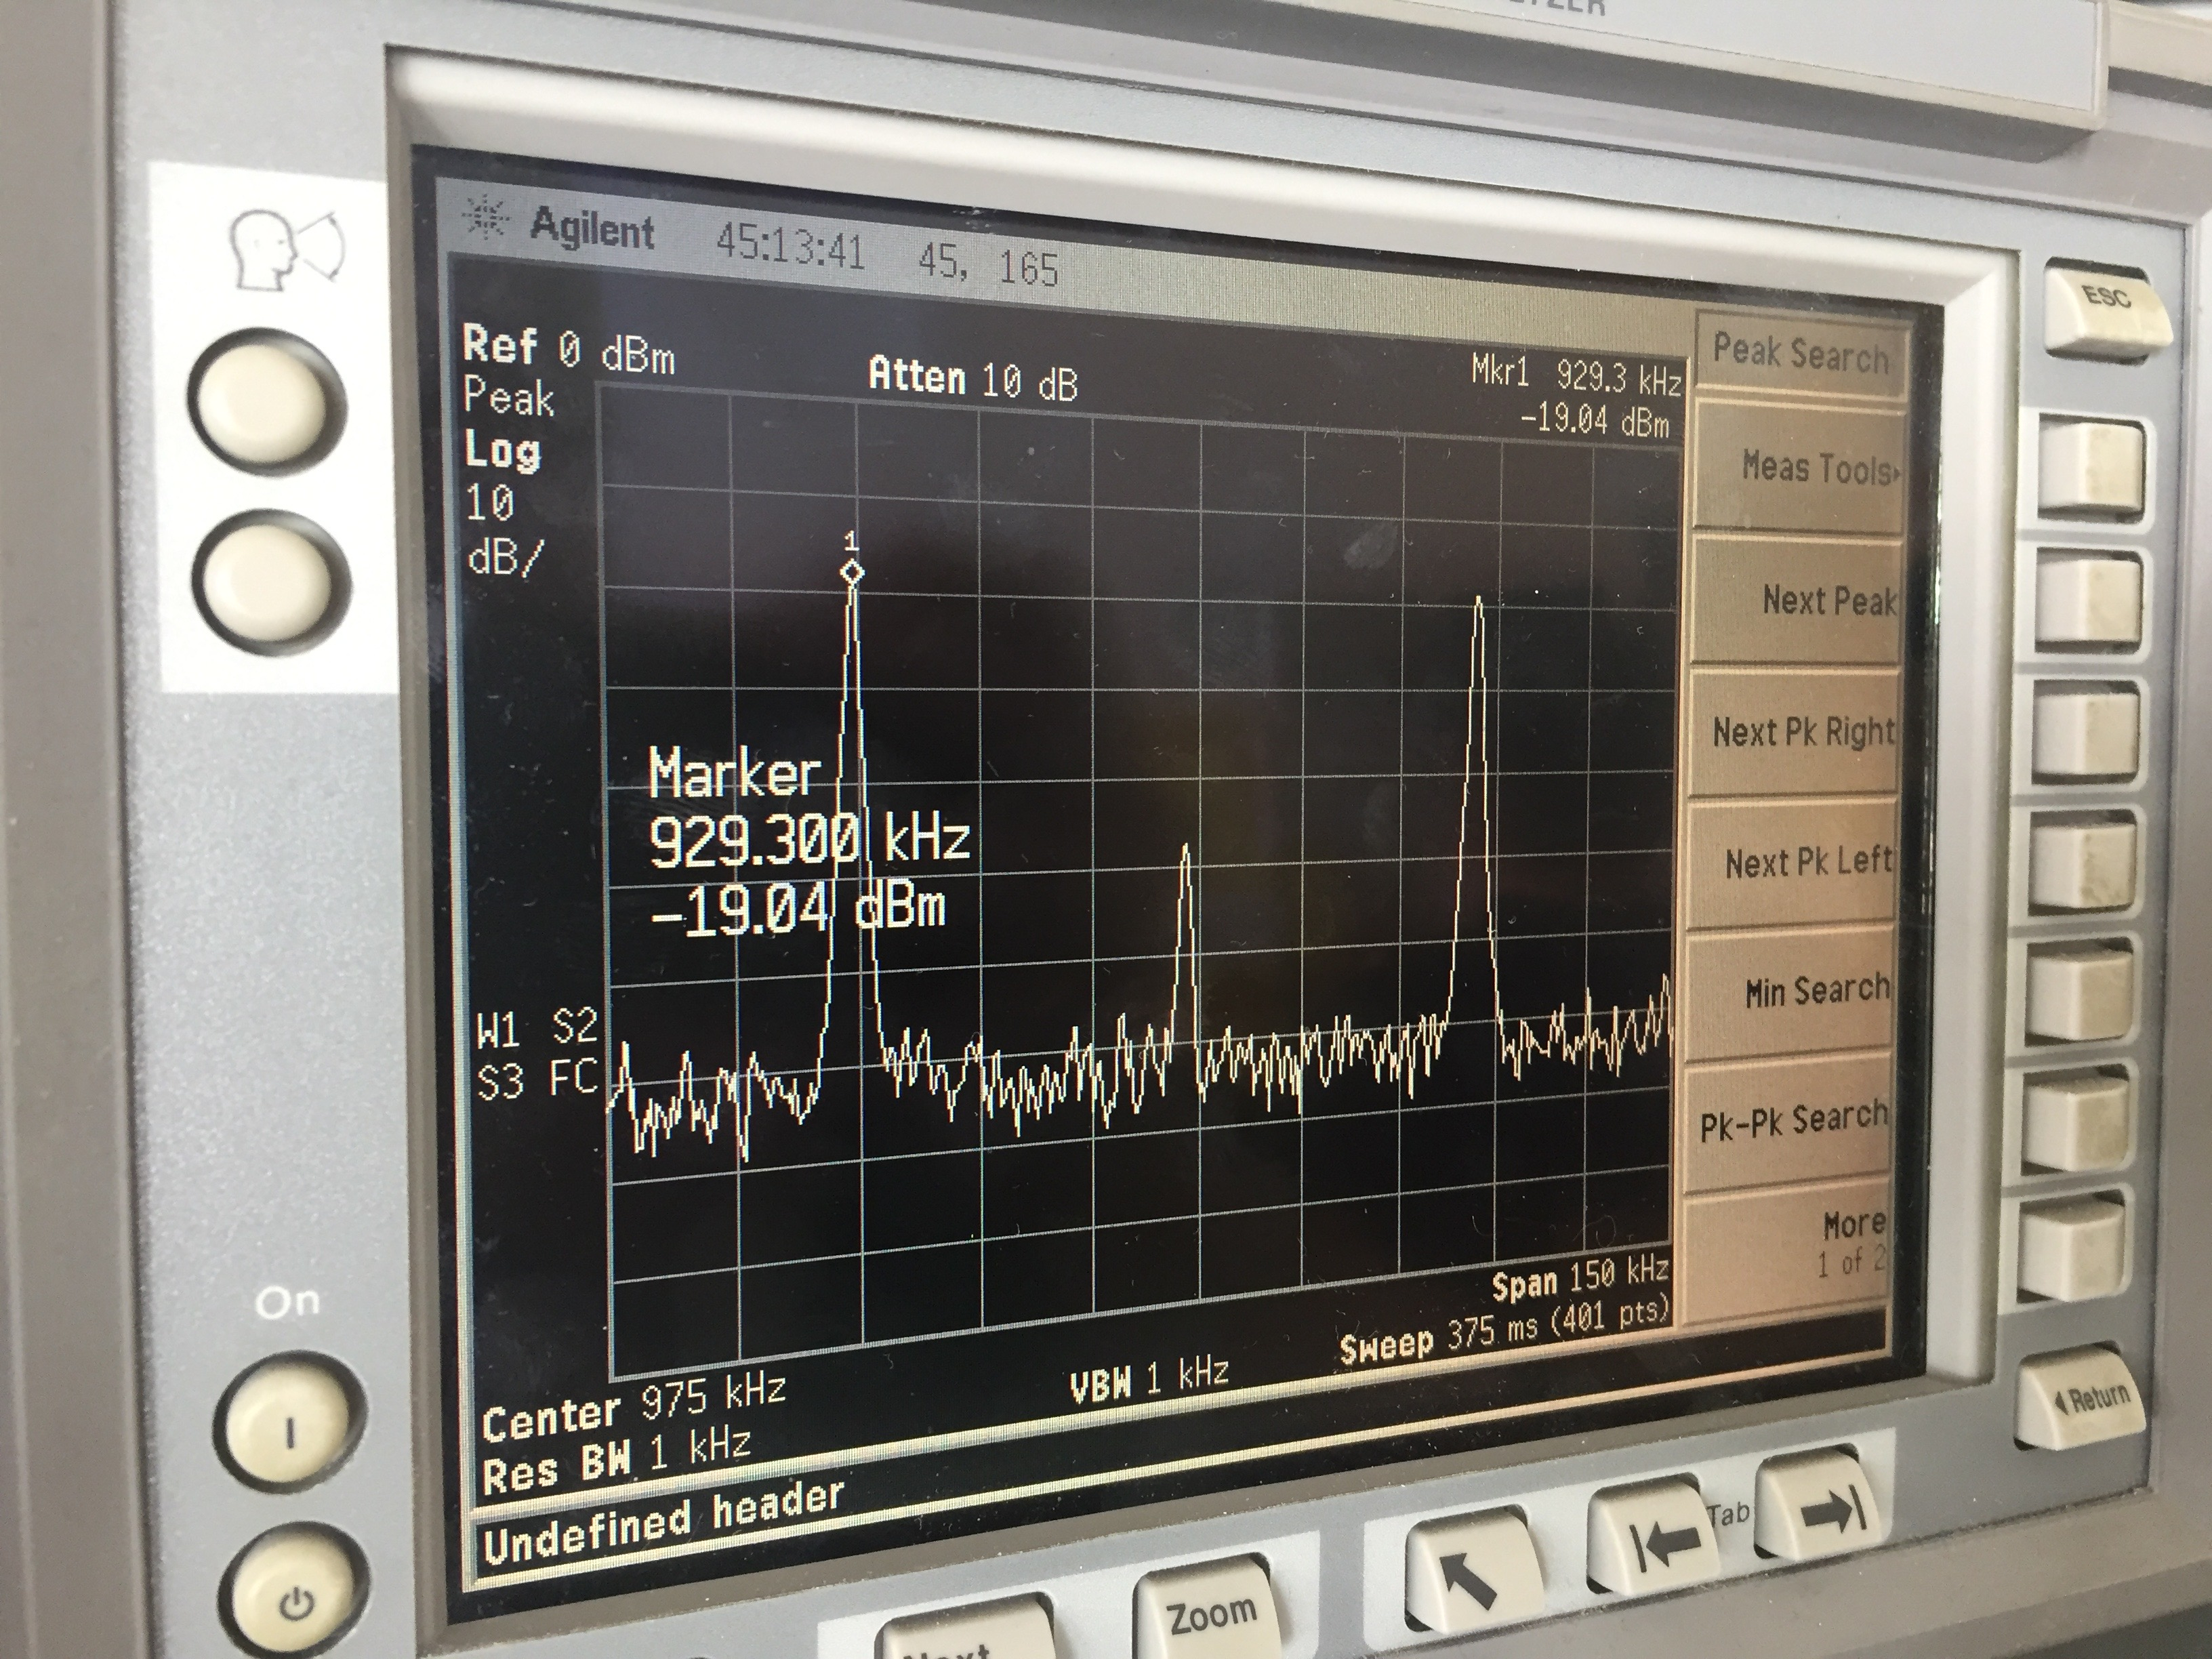
\includegraphics[width=\textwidth]{Spektrum_Pics/b1.jpg}
  \caption{Spektrum der mit dem Ringmodulator amplitudenmodulierten Schwingung mit Markierung vom Peak $\omega_\text{T} - \omega_\text{M}$}
  \label{fig:b1}
\end{figure}
\begin{figure}[H]
  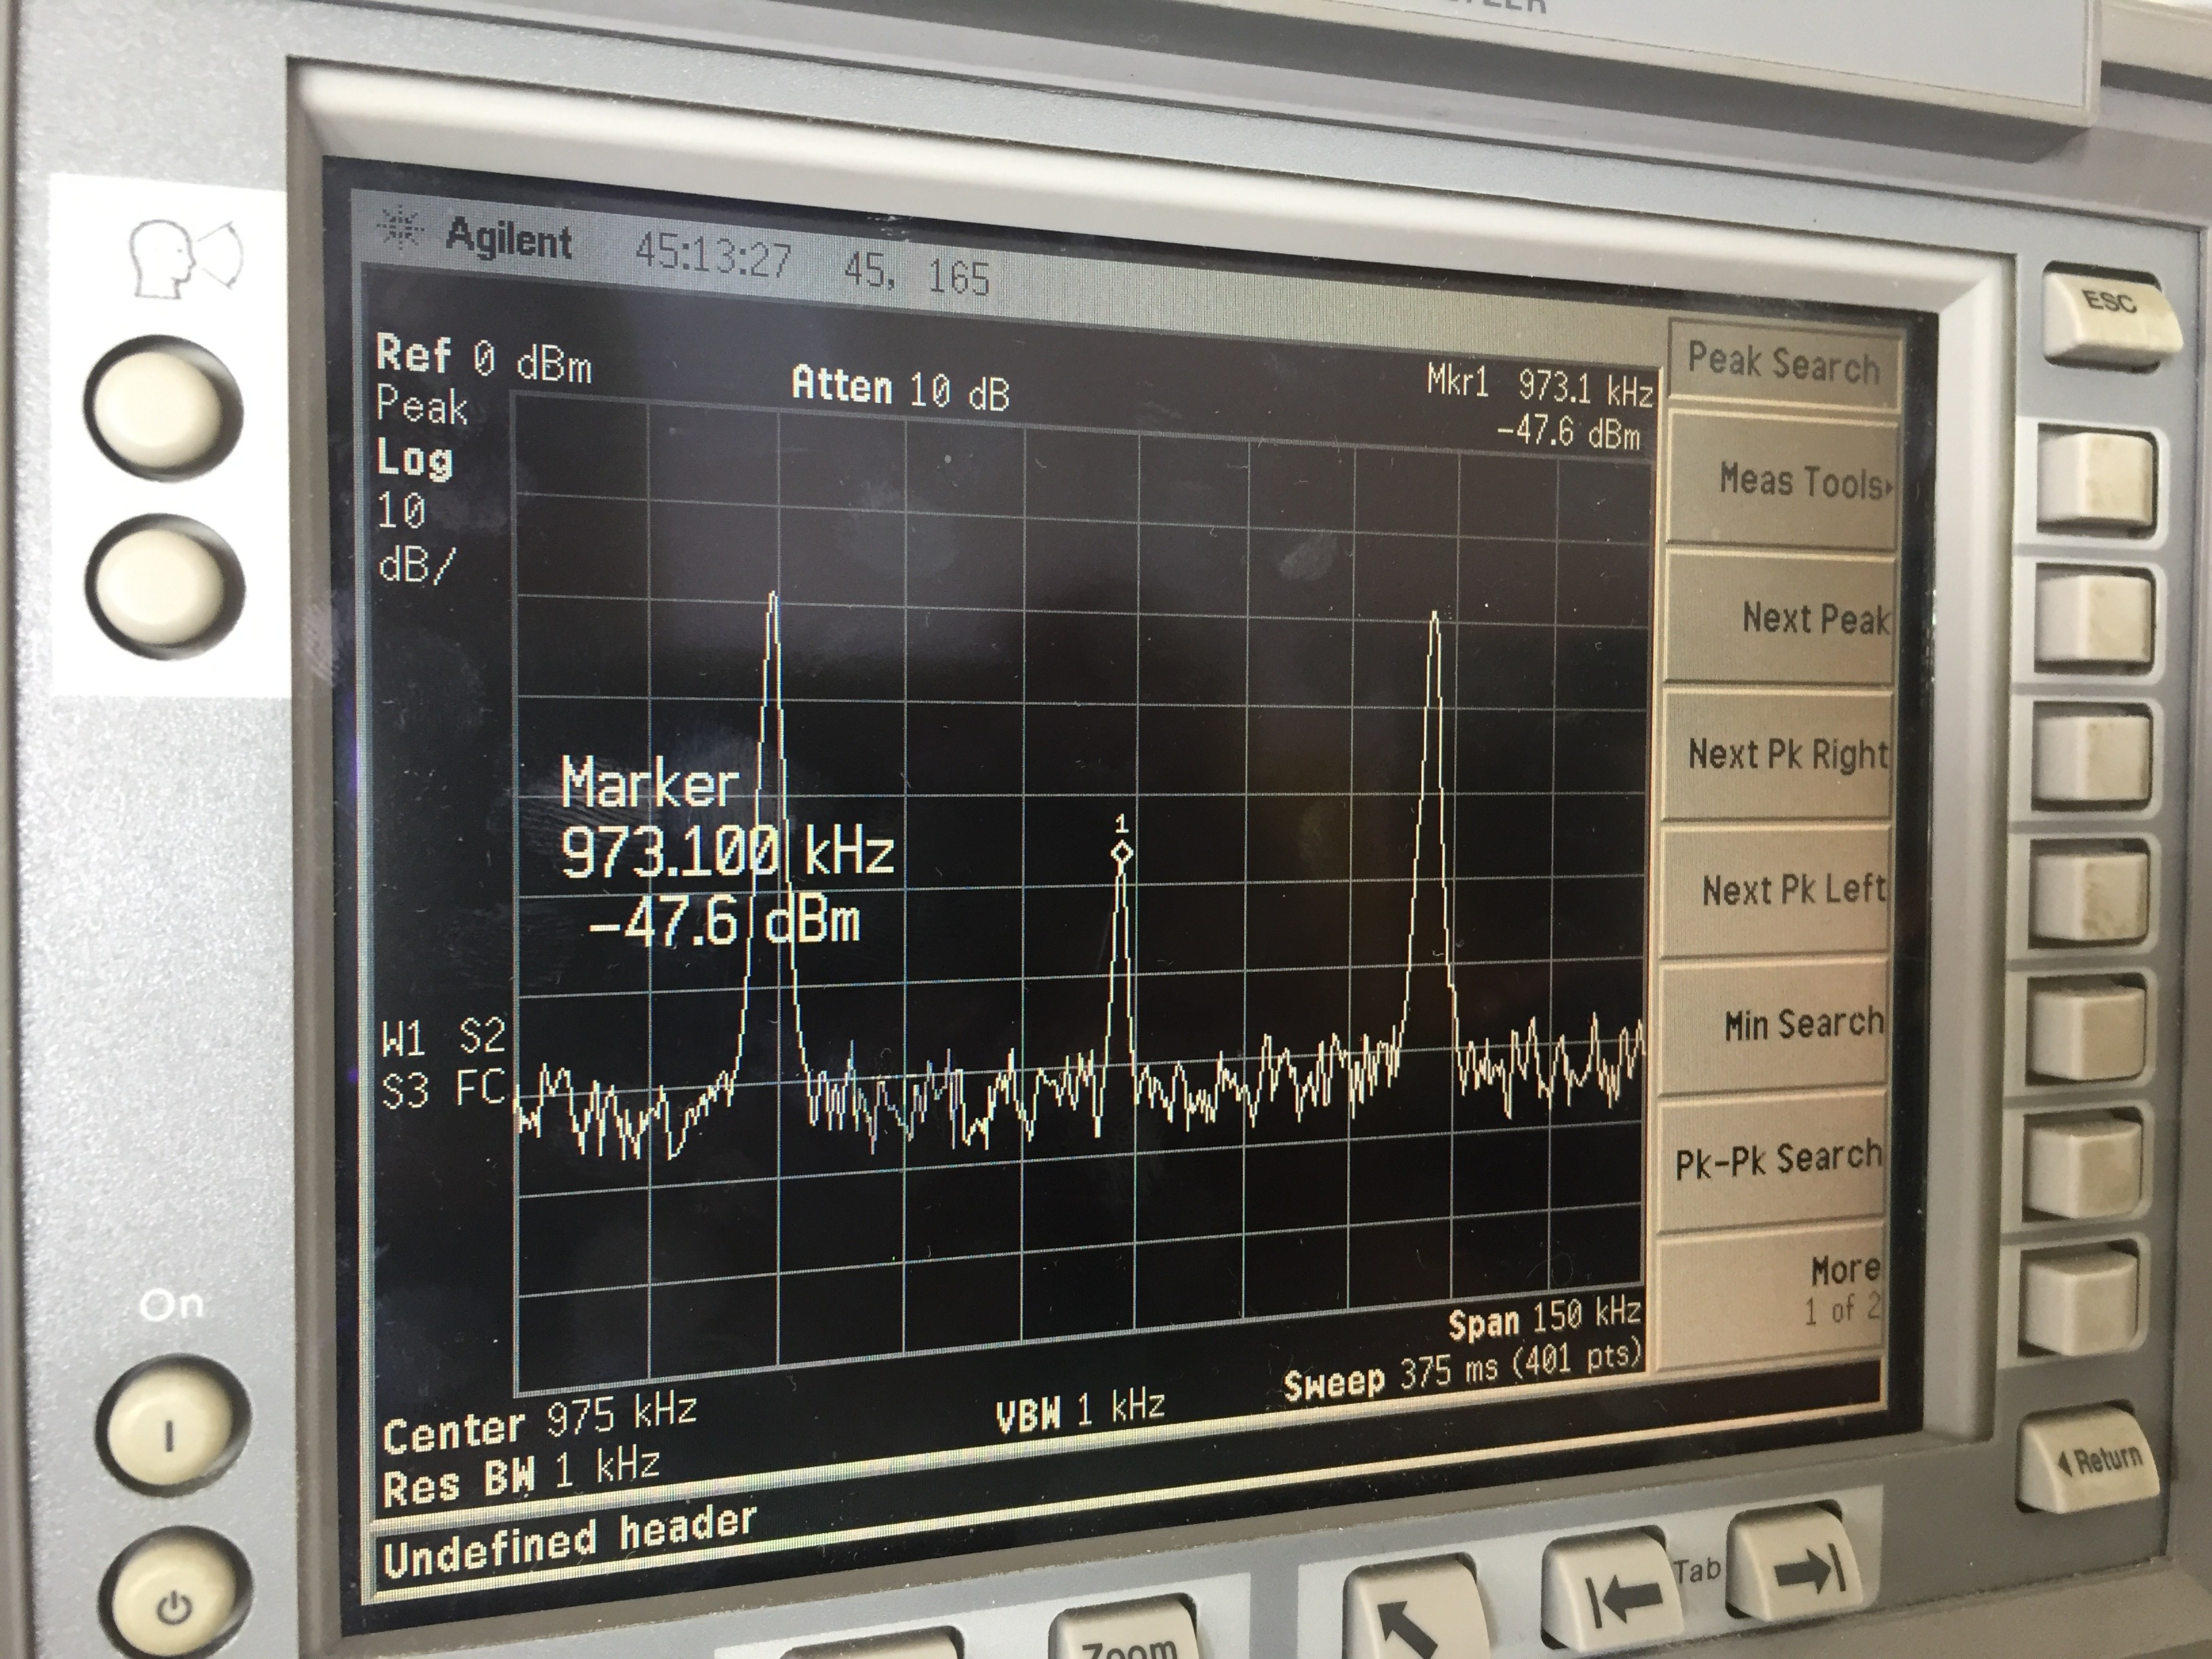
\includegraphics[width=\textwidth]{Spektrum_Pics/b2.jpg}
  \caption{Spektrum der mit dem Ringmodulator amplitudenmodulierten Schwingung mit Markierung vom Peak $\omega_\text{T}$}
  \label{fig:b2}
\end{figure}
\begin{figure}[H]
  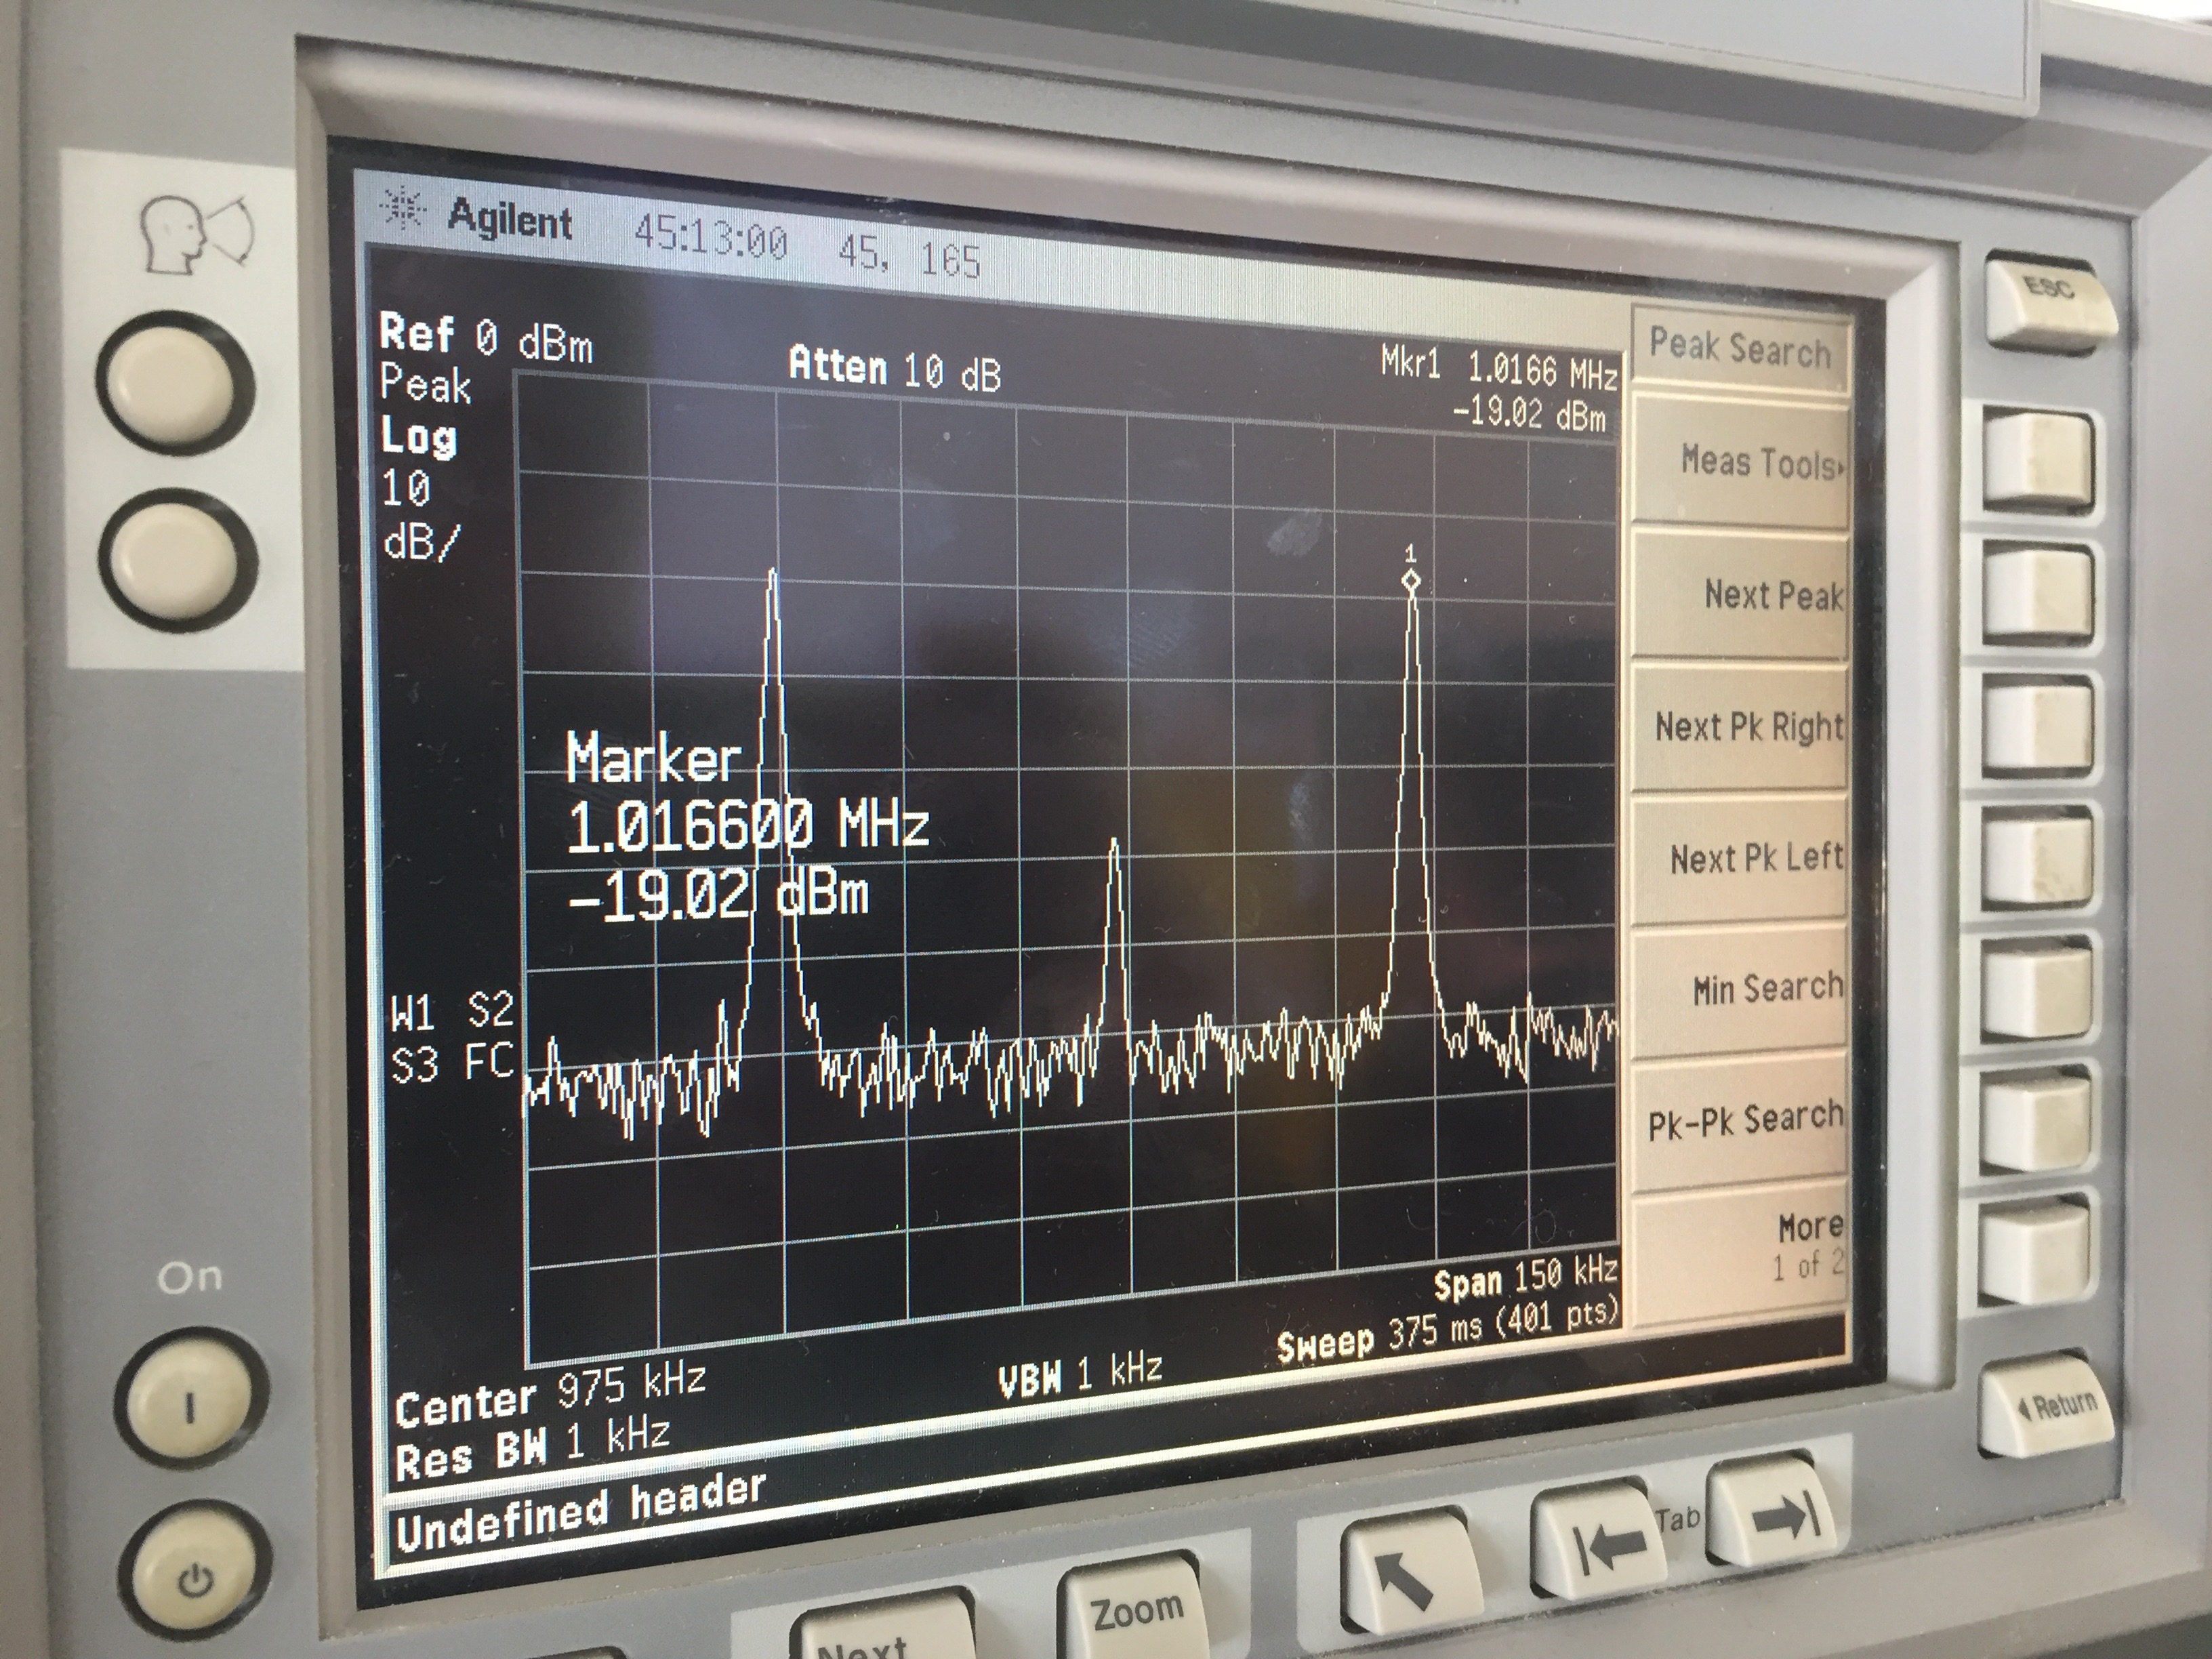
\includegraphics[width=\textwidth]{Spektrum_Pics/b3.jpg}
  \caption{Spektrum der mit dem Ringmodulator amplitudenmodulierten Schwingung mit Markierung vom Peak $\omega_\text{T} + \omega_\text{M}$}
  \label{fig:b3}
\end{figure}

Die aus dem Frequenzspektrum abgelesenen Frequenzen für die drei größten Peaks sind:
\begin{align*}
  \omega_1 &= \SI{929.3}{\kilo\hertz} & \omega_2 &= \SI{973.1}{\kilo\hertz} & \omega_3 &= \SI{1016.6}{\kilo\hertz}.\\
\end{align*}
Die Abweichungen zu den erwarteten Werten betragen:
\begin{align*}
  \frac{|(\omega_\text{T} - \omega_\text{M}) - \omega_1|}{\omega_\text{T} - \omega_\text{M}} &= \SI{0.3(1)}{\percent}\\
  \frac{|\omega_\text{T} - \omega_2|}{\omega_\text{T}} &= \SI{0.3(1)}{\percent}\\
  \frac{|(\omega_\text{T} + \omega_\text{M}) - \omega_3|}{\omega_\text{T} + \omega_\text{M}} &= \SI{0.3(1)}{\percent}.
\end{align*}

\subsection{Amplitudenmodulierte Schwingung mit Diode}

Nach Schaltung aus Abbildung \ref{fig:???} wird hier der allgemeine Fall der Amplitudenodulation mit einer Diode gezeigt.

\begin{figure}[H]
  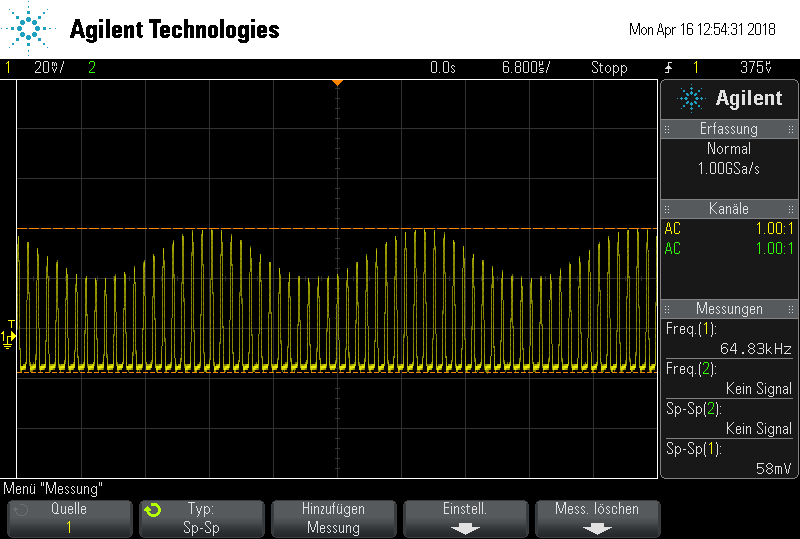
\includegraphics[width=\textwidth]{Oszi_Pics/amplModDiode.png}
  \caption{Amplitudenmodulierte Schwingung erzeugt mit einer Diode.}
  \label{fig:amplModDiode}
\end{figure}

Die so entstandene Schwebung ist in Abbildung \ref{fig:amplModDiode} zu sehen.



\subsection{Phasenzeugs}

\begin{figure}
  \centering
  \includegraphics{plotphase.pdf}
  \caption{Plot.}
  \label{fig:plot}
\end{figure}

Tabelle für copy and paste:
\begin{table}[h]
  \centering
  \begin{tabular}{S S}
    \toprule
    {$k$} & {$U\:/\:\si{\milli\volt}$}\\
    \midrule
    1 & 637.2\\
    3 & 212.4\\
    5 & 127.4\\
    7 & 91.03\\
    9 & 70.8\\
    \bottomrule
  \end{tabular}
  \caption{Amplituden Rechteckspannung.}
  \label{tab:rechtampl}
\end{table}
